


\begin{document}
This report describes the design, construction, and analysis of a discrete component operational amplifier. The topology chosen includes a cascoded current mirror that sinks current to an actively loaded differential pair amplifier which outputs single-endedly to a common source amplifier stage. This common source stage is then passed to an output Bipolar Junction Transistor (BJT) amplifier stage. The metal oxide semiconducting field effect transistors (MOSFET) in use are the ALD1106 for NMOS and the ALD1107 for PMOS. The general schematic for a generic op amp is shown in Figure \ref{fig:gen_schem}.

\begin{figure}[H]
    \begin{center}
    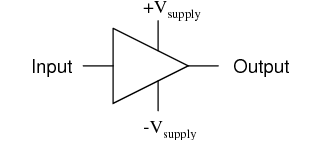
\includegraphics[scale=.45]{Introduction/genericopamp.png}
    \caption{General operational amplifier symbol \cite{b1}}
    \label{fig:gen_schem}
    \end{center}
    
\end{figure}
Operational amplifiers serve an integral building block for modern electronics. Op amps provide large gain with various configuration schema. This allows the circuit designer to use the op amp in different topologies and achieve different results, all without modifying the op amp circuit itself. In addition, an op amp provides significant gain while maintaining stability. The objective of this lab is to create an op amp out of discrete components that achieves the specifications as seen in Table \ref{tab:labspecs}.


\begin{table}[H]
\centering
\caption{Specifications}
\label{tab:labspecs}
\begin{tabular}{|l|l|}
\hline
\textbf{Specifications} &                 \\ \hline
Power                   & $\pm$5V         \\ \hline
Bias Current            & 500 $\mu$A      \\ \hline
Overall Voltage Gain    & 200V/V (46 dB)  \\ \hline
CMRR                    & $\geq$ 60dB     \\ \hline
Output Voltage Swing    & $\geq$ $\pm$ 2V \\ \hline
\end{tabular}
\end{table}

The input stage of an operational amplifier consists of a differential amplifier. Differential amplifiers are
desirable for their increased immunity to noise and that DC coupling of stages is possible without disturbing bias conditions. Each one of these designs will have some
advantage as well as some disadvantage over the other circuits. The primary function of the input
differential pair will be to provide a high common mode rejection ratio (CMRR). The differential gain,
$A_d$, need not be high, as long as the common mode gain, $A_{cm}$, is very small. This in turn is passed to an active load differential pair where the bulk of the differential gain will be achieved single endedly. The common source provides a final gain stage while reducing the effects of the output impedence of active load stage. 


\noindent Section 2 of this report describes the design, and when relevant, the simulations of the experiments. Experimental results and implementation are addressed in Section 3, including reasoning as to why a different circuit than the one outlined previously was constructed. A discussion of the results, sources of error, and areas of possible improvement are outlined in Section 4. Section 5 concludes this report. \newline

\end{document}